\section{ההתפלגות הנורמלית ושימוש בטבלת ה-Z}

\subsection{הגדרת שטחי הטבלה \foreignlanguage{english}{(Z, B, C)}}
הטבלה מחולקת לשלוש עמודות מרכזיות המאפשרות לנו למצוא הסתברויות ללא צורך בחישובים מורכבים של סימטריה:
\begin{description}
    \item[עמודה Z:] ציון התקן החיובי \LR{$z \ge 0$}. 
    \item[עמודה B:] השטח שבין הממוצע \LR{$0$} לבין ציון התקן \LR{$Z$}. 
    \item[עמודה C:] השטח שנמצא מעבר לציון התקן \LR{$Z$} (הזנב הקיצוני). 
\end{description}

\begin{figure}[H]
\centering
\begin{english}
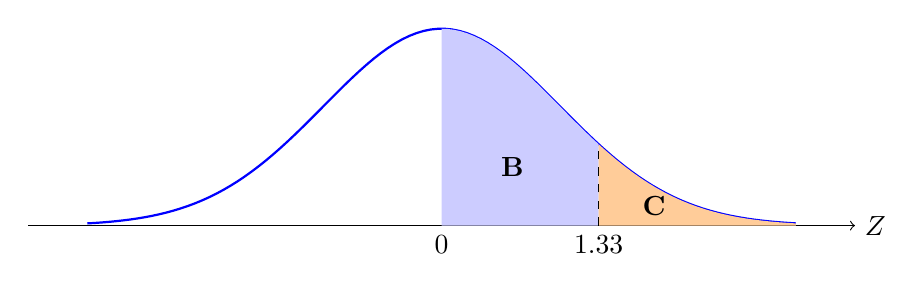
\begin{tikzpicture}[xscale=1.5, yscale=2.5]
  % עקומת הפעמון
  \draw[thick, blue, domain=-3:3, samples=100] plot (\x, {exp(-(\x*\x)/2)});
  \draw[->] (-3.5,0) -- (3.5,0) node[right] {$Z$};
  
  % שטח B (מהממוצע עד Z)
  \fill[blue!20] (0,0) -- plot[domain=0:1.33] (\x, {exp(-(\x*\x)/2)}) -- (1.33,0) -- cycle;
  \node at (0.6,0.3) {\textbf{B}};
  
  % שטח C (מה-Z עד אינסוף)
  \fill[orange!40] (1.33,0) -- plot[domain=1.33:3] (\x, {exp(-(\x*\x)/2)}) -- (3,0) -- cycle;
  \node at (1.8,0.1) {\textbf{C}};
  
  \draw[dashed] (1.33,0) -- (1.33,0.4);
  \node[below] at (0,0) {0};
  \node[below] at (1.33,0) {1.33};
\end{tikzpicture}
\end{english}
\caption{השטחים B ו-C לפי טבלת ההתפלגות הנורמלית.}
\end{figure}


\subsection{טבלת Z (מקטע מפורט)}
להלן המבנה המדויק של הטבלה כפי שמופיע בדף העזר למבחן:

\begin{center}
\begin{english} % מבטיח ש-Z יהיה משמאל והמספרים יוצגו נכון
\scriptsize 
\renewcommand{\arraystretch}{1.2}
\setlength{\tabcolsep}{4pt}
\rowcolors{2}{gray!10}{white} % צביעת שורות לנוחות קריאה
\begin{tabular}{|c|c|c||c|c|c||c|c|c||c|c|c|}
\hline
\rowcolor{gray!30}
\textbf{Z} & \textbf{B} & \textbf{C} & \textbf{Z} & \textbf{B} & \textbf{C} & \textbf{Z} & \textbf{B} & \textbf{C} & \textbf{Z} & \textbf{B} & \textbf{C} \\ \hline
0.00 & .0000 & .5000 & 0.30 & .1179 & .3821 & 0.60 & .2257 & .2743 & 0.90 & .3159 & .1841 \\
0.01 & .0040 & .4960 & 0.31 & .1217 & .3783 & 0.61 & .2291 & .2709 & 0.91 & .3186 & .1814 \\
0.02 & .0080 & .4920 & 0.32 & .1255 & .3745 & 0.62 & .2324 & .2676 & 0.92 & .3212 & .1788 \\
0.03 & .0120 & .4880 & 0.33 & .1293 & .3707 & 0.63 & .2357 & .2643 & 0.93 & .3238 & .1762 \\
0.04 & .0160 & .4840 & 0.34 & .1331 & .3669 & 0.64 & .2389 & .2611 & 0.94 & .3264 & .1736 \\
0.05 & .0199 & .4801 & 0.35 & .1368 & .3632 & 0.65 & .2422 & .2578 & 0.95 & .3289 & .1711 \\
0.06 & .0239 & .4761 & 0.36 & .1406 & .3594 & 0.66 & .2454 & .2546 & 0.96 & .3315 & .1685 \\
0.07 & .0279 & .4721 & 0.37 & .1443 & .3557 & 0.67 & .2486 & .2514 & 0.97 & .3340 & .1660 \\
0.08 & .0319 & .4681 & 0.38 & .1480 & .3520 & 0.68 & .2517 & .2483 & 0.98 & .3365 & .1635 \\
0.09 & .0359 & .4641 & 0.39 & .1517 & .3483 & 0.69 & .2549 & .2451 & 0.99 & .3389 & .1611 \\ \hline
0.10 & .0398 & .4602 & 0.40 & .1554 & .3446 & 0.70 & .2580 & .2420 & 1.00 & .3413 & .1587 \\
0.11 & .0438 & .4562 & 0.41 & .1591 & .3409 & 0.71 & .2611 & .2389 & 1.10 & .3643 & .1357 \\
0.12 & .0478 & .4522 & 0.42 & .1628 & .3372 & 0.72 & .2642 & .2358 & 1.20 & .3849 & .1151 \\
0.20 & .0793 & .4207 & 0.50 & .1915 & .3085 & 0.80 & .2881 & .2119 & 1.30 & .4032 & .0968 \\ \hline
\end{tabular}
\end{english}
\end{center}

\subsection{כללי עבודה חשובים}
\begin{itemize}
    \item \textbf{מציאת Z לפי הסתברות}: אם נתונה רמת סמך של 95\%, נחפש בעמודה B את הערך $0.4750$ (חצי מהשטח המרכזי) ונקבל $Z=1.96$. 
    \item \textbf{ערכים שליליים}: בגלל הסימטריה, השטח שבין $Z=-1$ ל-$0$ שווה בדיוק לשטח B עבור $Z=1$. 
    \item \textbf{הסתברות מצטברת ($\Phi$)}: כדי למצוא את כל השטח משמאל ל-$Z$ חיובי, נבצע חישוב של $0.5 + B$. 
\end{itemize}